\documentclass[titlepage, letterpaper, fleqn]{article}
\usepackage[utf8]{inputenc}
\usepackage{fancyhdr} % fancy headers, of course!
\usepackage{amsmath} % what do you think?
\usepackage{amsthm} % theorems!
\usepackage{extramarks} % more cute things
\usepackage{enumitem} % i'm not sure...
\usepackage{multicol} % multicolumn...?
\usepackage{amssymb} % more symbols
\usepackage{booktabs} % cool looking tables
\usepackage{tikz}

\topmargin=-0.45in
\evensidemargin=0in
\oddsidemargin=0in
\textwidth=6.5in
\textheight=9.0in
\headsep=0.25in


%
% You should change this things~
%

\newcommand{\mahteacher}{Dr. Viacheslav Kalashnikov}
\newcommand{\mahclass}{Applied Mathematics}
\newcommand{\mahtitle}{Activity 3}
\newcommand{\mahdate}{August 31, 2016}
\newcommand{\spacepls}{\vspace{5mm}}
\renewcommand\qedsymbol{\(\blacksquare\)}

%
% Header markings
%

\pagestyle{fancy}
\lhead{1170065 - Xavier Sánchez}
\chead{}
\rhead{}
\lfoot{}
\rfoot{}


\renewcommand\headrulewidth{0.4pt}
\renewcommand\footrulewidth{0.4pt}

\setlength\parindent{0pt}


%
% Create Problem Sections (stolen directly from jdavis/latex-homework-template @ github!)
%

\newcommand{\enterProblemHeader}[1]{
\nobreak\extramarks{}{Problem \arabic{#1} continued on next page\ldots}\nobreak{}
\nobreak\extramarks{Problem \arabic{#1} (continued)}{Problem \arabic{#1} continued on next page\ldots}\nobreak{}
}

\newcommand{\exitProblemHeader}[1]{
\nobreak\extramarks{Problem \arabic{#1} (continued)}{Problem \arabic{#1} continued on next page\ldots}\nobreak{}
\stepcounter{#1}
\nobreak\extramarks{Problem \arabic{#1}}{}\nobreak{}
}

\setcounter{secnumdepth}{0}
\newcounter{partCounter}
\newcounter{homeworkProblemCounter}
\setcounter{homeworkProblemCounter}{1}
\nobreak\extramarks{Exercise \arabic{homeworkProblemCounter}}{}\nobreak{}

% Alias for the Solution section header
\newcommand{\solution}{\textbf{\Large Solution}}

%Alias for the new step section
\newcommand{\steppy}[1]{\textbf{\large #1}}

%
% Homework Problem Environment
%
% This environment takes an optional argument. When given, it will adjust the
% problem counter. This is useful for when the problems given for your
% assignment aren't sequential. See the last 3 problems of this template for an
% example.
%
\newenvironment{homeworkProblem}[1][-1]{
\ifnum#1>0
\setcounter{homeworkProblemCounter}{#1}
\fi
\section{Exercise \arabic{homeworkProblemCounter}}
\setcounter{partCounter}{1}
\enterProblemHeader{homeworkProblemCounter}
}{
\exitProblemHeader{homeworkProblemCounter}
}

%
% Venn diagrams defs
%

\def\firstcircle{(0,0) circle (1.5cm)}
\def\secondcircle{(0:2cm) circle (1.5cm)}
\colorlet{circle edge}{blue!50}
\colorlet{circle area}{blue!20}

\tikzset{filled/.style={fill=circle area, draw=circle edge, thick},
    outline/.style={draw=circle edge, thick}}

%
% My actual info
%

\title{
\vspace{1in}
\textbf{Tecnológico de Monterrey} \\
\vspace{0.5in}
\textmd{\mahclass} \\
\large{\textit{\mahteacher}} \\
\vspace{0.5in}
\textsc{\mahtitle}\\
\textsc{1.1.1: Boolean operations on sets}\\
\author{01170065  - MIT \\
Xavier Fernando Cuauhtémoc Sánchez Díaz \\
\texttt{mail@gmail.com}}
\date{\mahdate}
}

\begin{document}

\begin{titlepage}
\maketitle
\end{titlepage}

%
% Actual document starts here~
%

{\large \textbf{a)} Show that for any \(x, x \in A + B\) iff \(x\) is an element of exactly one of A, B.}

\begin{proof}
  Assume \(x \in A + B\).

  \begin{align*}
  A + B &= (A-B) \cup (B-A)     &&\text{by definition}
  \\ &= (A \cap B^C) \cup (A^C \cap B)  &&\text{by complement}
  \end{align*}

  So \(x \in A \cap B^C\) or \(x \in A^C \cap B\). \\
  If \(x \in A \cap B^C\), then \(x \in A\) and \(x \not \in B\), since \(A \cap B^C \subseteq A\) and \(A \cap B^C \not \subseteq B\). \\
  If \(x \in A^C \cap B\), then \(x \in B\) and \(x \not \in A\), since \(A^C \cap B \subseteq B\) and \(A^C \cap B \not \subseteq A\).
\end{proof}

\spacepls

{\large \textbf{b)} Draw a Venn diagram for the operation (and use it to help intuition in what follows).}

\spacepls

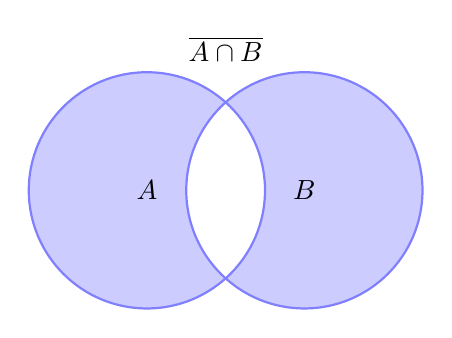
\begin{tikzpicture}
\draw[filled, even odd rule] \firstcircle node {$A$}
                             \secondcircle node{$B$};
\node[anchor=south] at (current bounding box.north) {$\overline{A \cap B}$};
\end{tikzpicture}

\spacepls

{\large \textbf{c)} Show that \(A + B \subseteq A \cup B\).}

\begin{proof}
	Assume \(x \in A + B\).

  \begin{align*}
  A + B &= (A-B) \cup (B-A)     &&\text{by definition}
  \\ &= (A \cap B^C) \cup (A^C \cap B)  &&\text{by complement}
  \end{align*}

  So \(x \in A \cap B^C\) or \(x \in A^C \cap B\). \\
  If \(x \in A \cap B^C\), then \(x \in A\) and also \(x \in A \cup B\), since \(A \subseteq A \cup B\). \\
  If \(x \in A^C \cap B\), then \(x \in B\) and also \(x \in A \cup B\), since \(B \subseteq A \cup B\). \\
  Therefore, \(A + B \subseteq A \cup B\).
\end{proof}

\spacepls
{\large \textbf{d)} Show that \(A + B\) is disjoint from \(A \cap B\).}

\begin{proof}
	Assume \(x \in A + B\).

  \begin{align*}
  A + B &= (A-B) \cup (B-A)     &&\text{by definition}
  \\ &= (A \cap B^C) \cup (A^C \cap B)  &&\text{by complement}
  \end{align*}

  So \(x \in A \cap B^C\) or \(x \in A^C \cap B\). \\
  If \(x \in A \cap B^C\), then \(x \in A\) but \(x \not \in B\), so \(x \not \in A \cap B\). \\
  If \(x \in A^C \cap B\), then \(x \in B\) but \(x \not \in A\), so \(x \not \in A \cap B\). \\
  Therefore, \(A + B\) is disjoint from \(A \cap B\).
\end{proof}

\pagebreak
{\large \textbf{e)} Show that \(A + B = (A \cup B) - (A \cap B)\).}

\begin{proof}
	\begin{align*}
	& (A \cup B) - (A \cap B) =
	\\ &= (A \cup B) \cap (A \cap B)^C     &&\tag*{by complement}
	\\ &= (A \cup B) \cap (A^C \cup B^C) 	&&\tag*{by de Morgan}
	\\ &= ((A \cup B) \cap A^C) \cup ((A \cup B) \cap B^C) &&\tag*{distribute union}
	\\ &= ((A \cap A^C) \cup (B \cap A^C)) \cup ((A \cap B^C) \cup (B \cap B^C)) &&\tag*{distribute intersection}
	\\ &= (B \cap A^C) \cup (A \cap B^C) &&\tag*{by intersection with complement}
	\\ &= (A-B) \cup (B-A)	&&\tag*{by definition}
	\\ &= A + B
	\end{align*}

	\begin{align*}
	& A + B =
	\\ &= (A-B) \cup (B-A)	&&\tag*{by definition}
	\\ &= (B \cap A^C) \cup (A \cap B^C) &&\tag*{by intersection with complement}
	\\ &= ((A \cap A^C) \cup (B \cap A^C)) \cup ((A \cap B^C) \cup (B \cap B^C)) &&\tag*{distribute intersection}
	\\ &= ((A \cup B) \cap A^C) \cup ((A \cup B) \cap B^C) &&\tag*{distribute union}
	\\ &= (A \cup B) \cap (A^C \cup B^C) 	&&\tag*{by de Morgan}
	\\ &= (A \cup B) \cap (A \cap B)^C     &&\tag*{by complement}
	\\ &= (A \cup B) - (A \cap B) &&\qedhere
	\end{align*}
\end{proof}

\spacepls

{\large \textbf{f.i)} Prove symmetric difference is associative: \((A + B) + C = A + (B + C)\)}

\begin{proof}
First, expand LHS:
\begin{align*}
	& (A + B) + C =
	\\ &= (((A \cap B^C) \cup (A^C \cap B))\cap C^C) \cup ((A + B)^C \cap C)
\end{align*}
by definition and complement,
\[= (((A \cap B^C) \cup (A^C \cap B))\cap C^C) \cup (((A \cup B) \cap (A^C \cup B^C))^C \cap C)\]
replacing \(A + B\) by another definition, \((A \cup B) \cap (A^C \cup B^C)\),
\[= (A \cap B^C \cap C^C) \cup (A^C \cap B \cap C^C) \cup (((A \cup B)^C\cup (A^C \cup B^C)^C) \cap C)\]
distributing intersection over union, and using de Morgan,
\[= (A \cap B^C \cap C^C) \cup (A^C \cap B \cap C^C) \cup (((A^C \cap B^C) \cup (A \cap B))\cap C)\]
by de Morgan,
\[= (A \cap B^C \cap C^C) \cup (A^C \cap B \cap C^C) \cup (A^C \cap B^C \cap C) \cup (A \cap B \cap C)\]
by distributing intersection over union.

\spacepls

Now expand RHS:
\begin{align*}
	& A + (B + C) =
	\\ &= (A \cap (B + C)^C) \cup (A^C \cap ((B \cap C^C) \cup (B^C \cap C)))
\end{align*}
by definition and complement,
\[= (A \cap ((B \cup C) \cap (B^C \cup C^C))^C) \cup (A^C \cap B \cap C^C) \cup (A^C \cap B^C \cap C)\]
replacing \(B + C\) by another definition, \((B \cup C) \cap (B^C \cup C^C)\), 
\[= (A \cap ((B \cup C)^C \cup (B^C \cup C^C)^C) \cup (A^C \cap B \cap C^C) \cup (A^C \cap B^C \cap C)\]
by de Morgan and distributing intersection over union,
\[= (A \cap ((B^C \cap C^C) \cup (B \cap C)) \cup (A^C \cap B \cap C^C) \cup (A^C \cap B^C \cap C)\]
by de Morgan,
\[= (A \cap B^C \cap C^C) \cup (A \cap B \cap C) \cup (A^C \cap B \cap C^C) \cup (A^C \cap B^C \cap C^C)\]
by distributing intersection over union.\\
And since union is commutative, then LHS \(=\) RHS, and therefore, \((A + B) + C = A + (B + C)\).
\end{proof}

\spacepls

{\large \textbf{f.ii)} Prove symmetric difference is commutative: \(A + B = B + A\)}

\begin{proof}
\begin{align*}
	& A + B =
	\\ &= (A - B) \cup (B - A)	&&\tag*{by definition}
	\\ &= (B - A) \cup (A - B) 	&&\tag*{by union commutativity}
	\\ &= B + A	&&\tag*{by definition}
\end{align*}
\end{proof}

\spacepls

{\large \textbf{f.iii)} Prove distribution of \(\cap\) over \(+\): \((A + B) \cap X = (A \cap X) + (B \cap X)\)}

\begin{proof}
First, expand LHS:
\begin{align*}
	& (A + B) \cap X =
	\\ &= ((A \cap B^C) \cup (A^C \cap B)) \cap X &&\tag*{by definition}
	\\ &= (A \cap B^C \cap X) \cup (A^C \cap B \cap X) &&\tag*{by distribution}
\end{align*}

\spacepls

Now expand RHS:
\begin{align*}
& (A \cap X) + (B \cap X) =
\\ &= ((A \cap X) \cap (B \cap X)^C) \cup ((A \cap X)^C \cap (B \cap X)) &&\tag*{by definition}
\\ &= ((A \cap X) \cap (B^C \cup X^C)) \cup ((A^C \cup X^C) \cap (B \cap X)) &&\tag*{by de Morgan}
\\ &= (A \cap x \cap B^C) \cup (A \cap X \cap X^C) \cup (A^C \cap B \cap X) \cup (B \cap X \cap X^C) &&\tag*{by distribution}
\\ &= (A \cap B^C \cap X) \cup (A^C \cap B \cap X) &&\tag*{by intersection with complement}
\end{align*}

And since LHS \(=\) RHS, therefore \((A + B) \cap X = (A \cap X) + (B \cap X)\).
\end{proof}

\pagebreak

{\large \textbf{f.iv)} Prove distribution of \(+\) over \(\cap\): \((A \cap B) + X = (A + X) \cap (B + X)\)}
\begin{proof}
Let \(A = \{1, 2, 3, 4\}, B = \{1, 3, 5, 7\}, X = \{1, 2, 4, 6\}\).
\[A \cap B = \{1, 3\}\]
\[(A \cap B) + X = \{2, 3, 4, 6\}\]
\[A + X = \{3, 6\}\]
\[B + X = \{2, 3, 4, 5, 6, 7\}\]
\[(A + X) \cap (B + X) = \{3, 6\}\]
Therefore, \((A \cap B) + X \not = (A + X) \cap (B + X)\).
\end{proof}

\spacepls

{\large \textbf{g)} Express \(-(A+B)\) using union, intersection and complement.}

\begin{align*}
	& -(A + B) =
	\\ &= (A + B)^C
	\\ &= ((A \cap B^C) \cup (A^C \cup B))^C
	\\ &= (A \cap B^C)^C \cap (A^C \cap B)^C
	\\ &= (A^C \cup B) \cap (A \cup B^C) \tag*{\(\square\)}
\end{align*}

\spacepls

{\large \textbf{h)} We have seen that each of intersection, union and difference corresponds to a truth-functional logical connective. To what connective mentioned in this chapter does symmetric difference correspond? Draw its truth table.}

\spacepls

The corresponding logical connective is often called \textbf{XOR}, which stands for \textit{Exclusive OR}: one of the two inputs must be true, but not both.

\begin{table}[h!]
\centering
\begin{tabular}{@{}ccc@{}}
\toprule
$\alpha$ & $\beta$ & $\alpha \oplus \beta$ \\ \midrule
1 & 1 & 0 \\
1 & 0 & 1 \\
0 & 1 & 1 \\
0 & 0 & 0 \\ \bottomrule
\end{tabular}
\end{table}

\end{document}